\documentclass{standalone}
\usepackage{amsmath,amssymb}
\usepackage[dvipsnames]{xcolor}
\usepackage{tikz} 
\usetikzlibrary{arrows, decorations.markings,decorations.pathreplacing,angles,quotes}
\usepackage{microtype}
\usepackage{fourier}

\definecolor{nb}{rgb}{0.12157, 0.46667, 0.705882}

%include other needed packages here   
\begin{document}

\begin{tikzpicture}
% include your tikz code here
    		\node[anchor=south west,inner sep=0] (Bild) at (0,0) {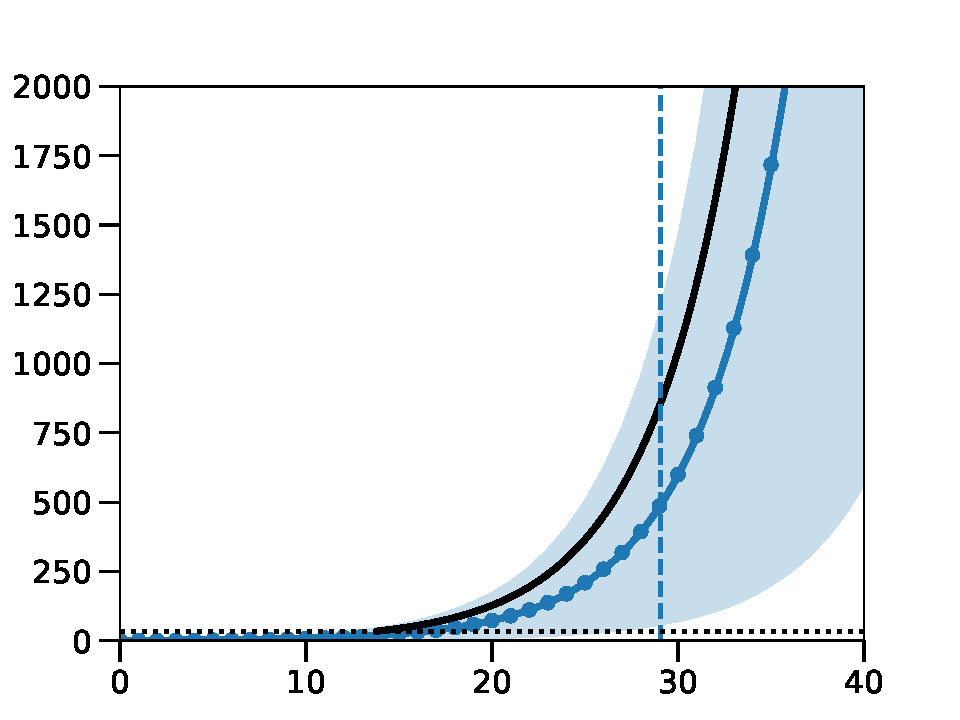
\includegraphics[scale=0.39]{fig6_blank.pdf}};
   		\begin{scope}[x=(Bild.south east),y=(Bild.north west)]

        	\draw (0.55,-0.01) node {time $t$ [days]};
        	\draw (-0.025,0.5) node [rotate=90] {epidemic size $I_{\text{surv}}(t)$};

        	\draw[color = nb, very thick] (0.925,0.675) -- node[right=6pt] {\color{black} \small Eq. (3)} (0.975,0.675);

        	\draw[color = black, very thick] (.925,0.8) -- (.975,0.8);
        	\node[right=2pt] at (0.975,.825) {\small Improved rule};
        	\node[right=2pt] at (0.975,0.775) {\small of thumb};
        	
        	\draw[color = black, very thick,dotted] (.925,0.55) -- (.975,0.55);
        	\node[right=2pt] at (0.975,.575) {\small Simple rule};
        	\node[right=2pt] at (0.975,0.525) {\small of thumb};

        	\draw[color = black] (0.55,0.82) node[right=0pt] {\small $\widehat{T}_{\text{hosp}}$};
        	
        	
        	\draw[color = nb] (0.925,0.3) node[right=0pt] {\large $\bullet$};
        	\node[right=2pt] at (0.975,0.33) {\small Simulation};
        	\node[right=2pt] at (0.975,0.27) {\small averages};
			
   		\end{scope}
\end{tikzpicture}

\end{document}